% ECE 228 - Team 17 - 3-minute presentation slides
% Beijing PM2.5 forecasting
%
% Compile with:  pdflatex slides.tex   (twice)
% Figures live in report/figures/ (populated by
%   python -m src.finish_run && python -m src.make_latex_tables
% from the project root).

\documentclass[10pt,aspectratio=169]{beamer}

\usepackage[T1]{fontenc}
\usepackage{lmodern}
\usepackage{booktabs}
\usepackage{amsmath}
\usepackage{graphicx}
\usepackage{xcolor}

\usetheme{Madrid}
\usecolortheme{seahorse}
\setbeamertemplate{navigation symbols}{}
\setbeamertemplate{footline}[frame number]

\graphicspath{{figures/}}

\title[PM2.5 Forecasting]{Short-term PM2.5 Forecasting on the Beijing\\Multi-Site Air Quality Dataset}
\subtitle{ECE 228, Team 17}
\author[Yu, Tsai]{Ting-Yu Yu \and Yun-Chen Tsai}
\institute[UCSD]{UC San Diego}
\date{Spring 2026}

\begin{document}

% --- Slide 1: Title --------------------------------------------------
\begin{frame}
\titlepage
\end{frame}


% --- Slide 2: Problem ------------------------------------------------
\begin{frame}{Why forecast PM2.5?}
\begin{columns}[T,onlytextwidth]
\begin{column}{0.58\linewidth}
\begin{itemize}\setlength\itemsep{0.35em}
  \item PM2.5 = fine particulate matter, the main driver of haze
        in dense cities; linked to respiratory and cardiovascular risk.
  \item $\geq 75\,\mu g/m^3$ is the WHO / Chinese GB
        \alert{``unhealthy''} threshold.
  \item Short-horizon forecasts let cities issue advisories
        \emph{before} a spike hits.
\end{itemize}
\vspace{0.5em}
\textbf{Two questions we set out to answer:}
\begin{enumerate}\setlength\itemsep{0.2em}
  \item Do sequence models (LSTM / GRU / Transformer)
        beat feature-based regressors here?
  \item Does context from the \emph{other} 11 stations help?
\end{enumerate}
\end{column}
\begin{column}{0.4\linewidth}
\small
\textbf{Data}\\
Beijing Multi-Site Air Quality (UCI):
\begin{itemize}\setlength\itemsep{0.1em}
  \item 12 monitoring stations
  \item hourly readings, 2013-03 -- 2017-02
  \item 6 pollutants + 6 weather variables
  \item $\sim$35\,000 hours per station
\end{itemize}
\vspace{0.4em}
\textbf{Target}\\
PM2.5 at $t{+}h$, $h \in \{1, 6\}$ hours ahead.
\end{column}
\end{columns}
\end{frame}


% --- Slide 3: Setup --------------------------------------------------
\begin{frame}{Setup: windows, splits, two input settings}
\begin{columns}[T,onlytextwidth]
\begin{column}{0.55\linewidth}
\small
\textbf{Sliding window}\\
Input: last 24 hours of (pollutants, weather, time, station).\\
Target: PM2.5 at $t{+}h$.
\vspace{0.5em}

\textbf{Time-based split} (no leakage)\\
\begin{tabular}{ll}
\toprule
Train & 2013-03 -- 2015-12 \\
Val   & 2016-01 -- 2016-06 \\
Test  & 2016-07 -- 2017-02 \\
\bottomrule
\end{tabular}
\vspace{0.5em}

\textbf{Preprocessing}\\
Standardize on train only; clip to $\pm 8\sigma$
(rainfall outliers were causing GRU NaN losses).\\
Cyclic $(\sin,\cos)$ encoding for wind direction, hour-of-day,
day-of-week, month-of-year.
\end{column}
\begin{column}{0.45\linewidth}
\small
\textbf{Two input settings}
\begin{itemize}\setlength\itemsep{0.25em}
  \item \alert{global} -- target station's own 24 h history;
        station id as embedding (DL) / one-hot (baselines).\\
        $F = 19$ features per timestep.
  \item \alert{multi-site} -- same as above, but every timestep
        also gets the channel-wise \emph{mean of the other 11
        stations}. Target station masked out (no leakage).\\
        $F = 38$ features per timestep.
\end{itemize}
\vspace{0.6em}

\textbf{Metrics}\\
MAE, RMSE, $R^2$, and \alert{spike-recall} = fraction of
test hours with $y \geq 75\,\mu g/m^3$ where the model also
predicts $\geq 75$ (i.e.\ would we have flagged it?).
\end{column}
\end{columns}
\end{frame}


% --- Slide 4: Models -------------------------------------------------
\begin{frame}{Seven models, one pipeline}
\small
\begin{tabular}{p{2.3cm}p{4.8cm}p{6.0cm}}
\toprule
\textbf{Family} & \textbf{Models} & \textbf{Notes} \\
\midrule
no learning   & \textbf{Persistence} ($\hat y_{t+h}=y_t$)
              & Tough baseline at $h{=}1$; collapses at $h{=}6$. \\
feature-based & \textbf{Ridge}, \textbf{Random Forest},
                \textbf{Gradient Boosting}
              & Flatten $24{\times}F$ window; append one-hot station id. \\
sequence      & \textbf{LSTM}, \textbf{GRU},
                \textbf{Transformer enc.}
              & 2 layers, hidden 128, dropout 0.2; 8-dim station embedding.\\
\bottomrule
\end{tabular}

\vspace{0.7em}
\textbf{Training (sequence models).}
AdamW (lr $10^{-3}$, weight decay $10^{-5}$), cosine LR,
batch 512, grad-clip 1.0, smooth-$L_1$ loss in standardized space,
max 15 epochs, early stop on val MAE (patience 4).
PyTorch MPS backend (Apple Silicon GPU).

\vspace{0.5em}
\textbf{Same data, same targets, same metrics} across all seven models
$\Rightarrow$ apples-to-apples comparison of model families
and of the two input settings.
\end{frame}


% --- Slide 5: Headline results ---------------------------------------
\begin{frame}{Result 1: GRU multi-site is the best at both horizons}
\begin{columns}[T,onlytextwidth]
\begin{column}{0.55\linewidth}
\centering
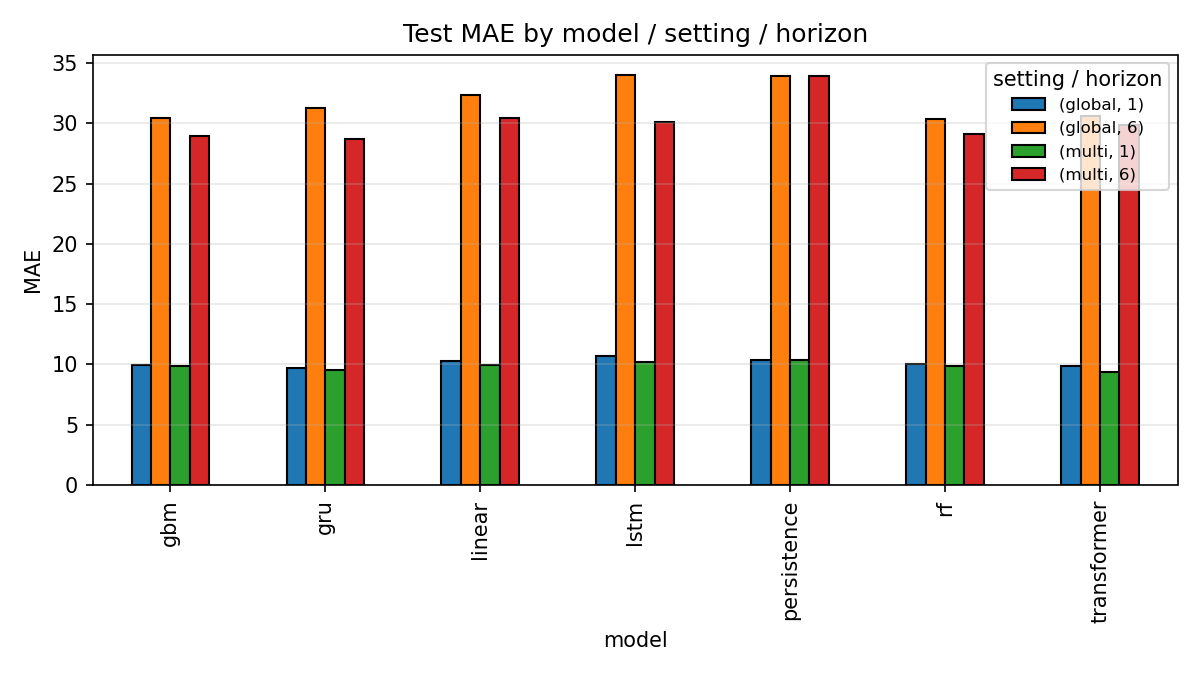
\includegraphics[width=\linewidth]{comparison_MAE.png}\\
{\footnotesize Test MAE per model / input setting / horizon
(lower is better).}
\end{column}
\begin{column}{0.42\linewidth}
\footnotesize
\textbf{1 hour ahead}\\
Persistence already gets $R^2\!\approx\!0.95$.
\textbf{Transformer multi-site MAE = 9.41}, \textbf{GRU multi-site = 9.51}
- both edge past every baseline.
Spike-recall \textbf{$\approx$ 0.95} ($\geq 75\,\mu g/m^3$).

\vspace{0.6em}
\textbf{6 hours ahead}\\
Persistence collapses ($R^2\!\approx\!0.56$).
\textbf{GRU multi-site MAE = 28.75} edges out the best
baseline (GBM multi-site, 29.00). LSTM struggles at our
default LR / patience.

\vspace{0.6em}
\alert{Take-away:} sequence models help most when paired
with the multi-site context.
\end{column}
\end{columns}
\end{frame}


% --- Slide 6: Multi-site context -------------------------------------
\begin{frame}{Result 2: a trivial spatial summary already helps}
\begin{columns}[T,onlytextwidth]
\begin{column}{0.45\linewidth}
\small
\textbf{Multi-site setting:} at every timestep feed the model
the channel-wise \emph{mean of the other 11 stations}.
\\Doubles $F$ from 19 to 38.\\
No graph, no attention -- the simplest possible spatial summary.

\vspace{0.6em}
\textbf{Test-MAE change vs.\ global ($\mu g/m^3$):}\\
\begin{tabular}{lrr}
\toprule
Model & $\Delta$ at $h{=}1$ & $\Delta$ at $h{=}6$ \\
\midrule
Ridge        & $-0.38$ & $-1.87$ \\
Random Forest& $-0.18$ & $-1.26$ \\
GBM          & $-0.11$ & $-1.43$ \\
GRU          & $-0.19$ & $\mathbf{-2.55}$ \\
Transformer  & $-0.43$ & $-0.79$ \\
\bottomrule
\end{tabular}

\vspace{0.4em}
Consistent across all models; \emph{larger} gains at $h{=}6$
where local history alone leaves more to predict.
A wind-aware aggregator should help more still.
\end{column}
\begin{column}{0.52\linewidth}
\centering
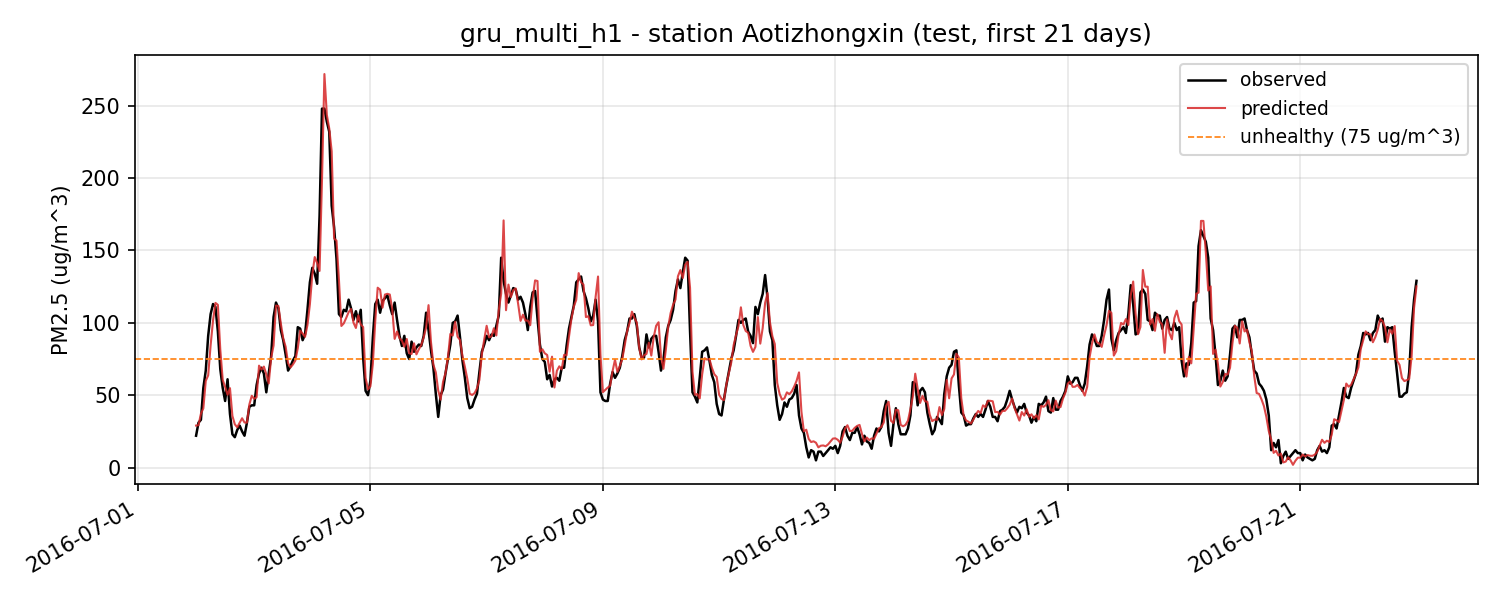
\includegraphics[width=\linewidth]{gru_multi_h1_timeseries.png}\\
\footnotesize
GRU (multi-site, $h{=}1$) at Aotizhongxin station, first three
weeks of test. Tracks the daily cycle and the multi-day haze
episodes; dashed orange = $75\,\mu g/m^3$ unhealthy threshold.
\end{column}
\end{columns}
\end{frame}


% --- Slide 7: Conclusion ---------------------------------------------
\begin{frame}{Wrap-up}
\begin{columns}[T,onlytextwidth]
\begin{column}{0.55\linewidth}
\textbf{What we found}
\begin{itemize}\setlength\itemsep{0.2em}
  \item At $h{=}1$, GRU / Transformer (multi-site) reach
        MAE $\approx 9.4$ and recall $\sim$\,95\% of unhealthy hours.
  \item At $h{=}6$, GRU (multi-site) is the best single model
        (MAE 28.75), narrowly above GBM (29.00).
  \item A trivial \emph{spatial mean} of the other 11 stations
        gives a consistent MAE boost - larger at $h{=}6$
        ($-1$ to $-4\,\mu g/m^3$).
\end{itemize}
\end{column}
\begin{column}{0.42\linewidth}
\textbf{Next steps}
\begin{itemize}\setlength\itemsep{0.2em}
  \item Wind-direction-aware spatial aggregation
        (upwind stations matter more).
  \item Proper LR / patience sweep tuned for $h{=}6$.
  \item Multi-task forecasting (PM10, NO$_2$, $\ldots$)
        for a shared representation.
\end{itemize}
\vspace{0.6em}
\textbf{Reproducible.} Code, training, evaluation, figures,
and the full report all live in the project repository.
\end{column}
\end{columns}
\vspace{0.8em}
\centering
\textit{Thanks -- questions?}
\end{frame}


\end{document}
